\section{WS1: Crazyflie Development environment}
This section introduces the Crazyflie development environment. This project was tested on Ubuntu 16.04.4 LTS and it assumes that the reader has this version installed.

\noindent Crazyflie development is split into client and firmware development. Crazyflie firmware is built and uploaded onto the drone while the client runs on a remote computer and is used to connect to the drone and control it.

\subsection{Setting PC permissions}
The following instructions are given as decribed in \cite{book_ros}.
Special PC permission need to be set before continuing as the CrazyRadio PA works only for a user with sudo rights. This requirement is eliminated by creating a \texttt{plugdev} group and add the current user to it.
\begin{mdframed}[backgroundcolor=light-gray, linecolor=light-gray]
  \texttt{\$ sudo groupadd plugdev}\\
  \texttt{\$ sudo usermod -a -G plugdev \$USER}
\end{mdframed}

\noindent Next a new udev-rule is created to allow members of the \texttt{plugdev} access the CrazyRadio PA.
\begin{mdframed}[backgroundcolor=light-gray, linecolor=light-gray]
  \texttt{\$ sudo nano /etc/udev/rules.d/99-crazyradio.rules}
\end{mdframed}

\noindent With the following content:
\begin{minted}[breaklines, linenos,frame=single]{bash}
# Crazyradio (normal operation)
SUBSYSTEM=="usb", ATTRS{idVendor}=="1915", ATTRS{idProduct}=="7777", MODE="0664", GROUP="plugdev"
# Bootloader
SUBSYSTEM=="usb", ATTRS{idVendor}=="1915", ATTRS{idProduct}=="0101", MODE="0664", GROUP="plugdev"
\end{minted}

\noindent To be able to use the CrazyFlie connected to the usb port, another udev-rule is created:
\begin{mdframed}[backgroundcolor=light-gray, linecolor=light-gray]
  \texttt{\$ sudo nano /etc/udev/rules.d/99-crazyflie.rules}
\end{mdframed}
With the following content:
\begin{minted}[breaklines, linenos,frame=single]{bash}
SUBSYSTEM=="usb", ATTRS{idVendor}=="0483", ATTRS{idProduct}=="5740", MODE="0664", GROUP="plugdev"
\end{minted}

The last step is to reload the udev rules as follows:
\begin{mdframed}[backgroundcolor=light-gray, linecolor=light-gray]
    \begin{verbatim}
$ sudo udevadm control --reload-rules
$ sudo udevadm trigger
    \end{verbatim}
\end{mdframed}

To enable the newly created rules the user must log-out and log-in into the system. Once done the CrazyRadio PA and the CrazyFlie usb connection can be used without superuser access.

\subsection{Crazyflie client}
The CrazyFlie client is a GUI application built on top of \texttt{crazyflie-lib-python}, a Python library allowing the control of the crazyflie from a remote PC. This project requires both components therefore this section starts with the installation of \texttt{crazyflie-lib-python}.
At first install the required dependencies:

\begin{mdframed}[backgroundcolor=light-gray, linecolor=light-gray]
\begin{Verbatim}
$ sudo apt-get install git python3 python3-pip python3-pyqt5 \
    python3-pyqt5.qtsvg python3-numpy python3-zmq
$ sudo pip3 install pyusb==1.0.0b2
$ sudo pip3 install pyqtgraph appdirs
\end{Verbatim}
\end{mdframed}

The issue the following commands to install \texttt{crazyflie-lib-python} in the \url{~/crazyflie} directory:
\begin{mdframed}[backgroundcolor=light-gray, linecolor=light-gray]
\begin{Verbatim}
$ mkdir ~/crazyflie
$ cd ~/crazyflie
$ git clone https://github.com/bitcraze/crazyflie-lib-python.git
$ cd crazyflie-lib-python
$ pip3 install --user -e .
\end{Verbatim}
\end{mdframed}
The \texttt{crazyflie-lib-python} library uses Python3, hence the use of \texttt{pip3} for package installation.

The next step is to install the Crazyflie client. The following commands install the client and all of it's dependencies:
\begin{mdframed}[backgroundcolor=light-gray, linecolor=light-gray]
\begin{Verbatim}
$ cd ~/crazyflie
$ https://github.com/bitcraze/crazyflie-clients-python.git
$ cd crazyflie-clients-python
$ pip3 install --user -e .
\end{Verbatim}
\end{mdframed}

At this point the CrazyFlie client can be started as such:
\begin{mdframed}[backgroundcolor=light-gray, linecolor=light-gray]
\begin{Verbatim}
$ cd ~/crazyflie/crazyflie-clients-python
$ python3 bin/cfclient
\end{Verbatim}
\end{mdframed}

This will start the CrazyFlie Client GUI as seen below.

\begin{figure}[H]
\centering
 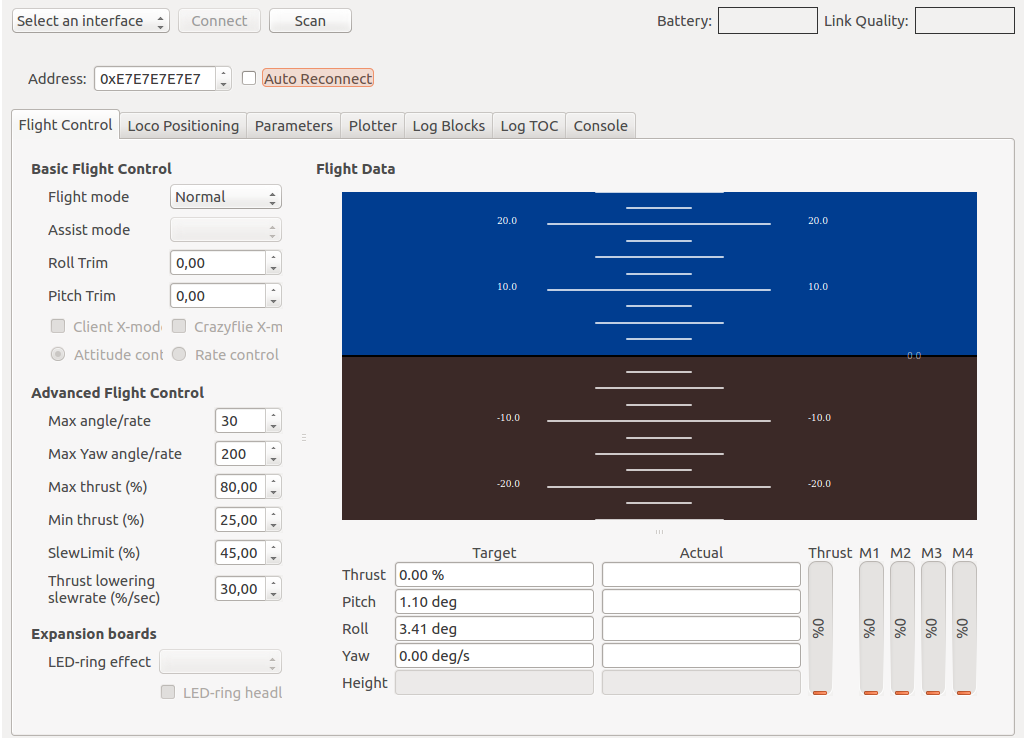
\includegraphics[scale=0.25]{pc-client.png}
 \caption{The CrazyFlie PC client}
 \label{figure:crazyflie_client}
\end{figure}

 If the address of the drone hasn't been previously modified and the CrazyRadio PA is attached to the PC, the user can press the \texttt{Scan} button which shows available CrazyFlies. Selecting an available drone and clicking the \texttt{Connect} button, connects and displays the state of the drone such as attitude, battery level and the signal quality.

\subsection{Crazyflie firmware}
This section describes how to build and upload the firmware for a Crazyflie drone.
For the purpose of this project the firmware will be built with little modifications as most operations will be done by the client.\\

\noindent There are two firmwares that need to be built, namely NRF51 (power management and radio communication) and STM32 (main firmware). The working directory for Bitcraze Crazyflie is assumed to located at \url{~/crazyflie}.

\subsubsection{Building and uploading STM32 firmware}
\noindent Instructions are given according to Bitcraze firmware GitHub \cite{web_bitcraze_git_fw}\\
\noindent Install the ARM toolchain:
\begin{mdframed}[backgroundcolor=light-gray, linecolor=light-gray]
\begin{verbatim}
$ sudo add-apt-repository ppa:team-gcc-arm-embedded/ppa
$ sudo apt-get update
$ sudo apt-get install libnewlib-arm-none-eabi
\end{verbatim}
\end{mdframed}

Clone the repository into the user's home directory
\begin{mdframed}[backgroundcolor=light-gray, linecolor=light-gray]
\begin{verbatim}
$ cd ~/crazyflie
$ git clone --recursive https://github.com/bitcraze/crazyflie-firmware.git
\end{verbatim}
\end{mdframed}

Compile the firmware
\begin{mdframed}[backgroundcolor=light-gray, linecolor=light-gray]
\begin{verbatim}
$ cd ~/crazyflie/crazyflie-firmware
$ make
\end{verbatim}
\end{mdframed}


\noindent To upload the firmware on the Crazyflie it must be put in Bootloader mode. To do so, power it down then press and hold the power button for a few seconds until a blue led starts blinking, the release the power button. At this time two blue led's should be blinking. Make sure the CrazyRadio PA is connected to the computer and issue the following command:
\begin{mdframed}[backgroundcolor=light-gray, linecolor=light-gray]
\texttt{\$ make cload}
\end{mdframed}

\noindent At this point wait for the firmware to be flashed on the drone and it will automatically restart once finished.

\subsubsection{Building and uploading NRF51 firmware}
\noindent Instructions are given according to Bitcraze NRF51 firmware GitHub \cite{web_bitcraze_git_fw_nrf}\\

\noindent Install the required tools
\begin{mdframed}[backgroundcolor=light-gray, linecolor=light-gray]
\begin{verbatim}
$ sudo apt-get install gcc-arm-none-eabi gdb-arm-none-eabi \ 
        binutils-arm-none-eabi
\end{verbatim}
\end{mdframed}

Clone the repository into the user’s home directory
\begin{mdframed}[backgroundcolor=light-gray, linecolor=light-gray]
\begin{verbatim}
$ cd ~/crazyflie/
$ git clone https://github.com/bitcraze/crazyflie2-nrf-firmware.git
$ ./tools/build/download_deps
\end{verbatim}
\end{mdframed}
Compile and upload the firmware
\begin{mdframed}[backgroundcolor=light-gray, linecolor=light-gray]
\begin{Verbatim}
$ cd ~/crazyflie/crazyflie2-nrf-firmware
$ make
## Put CrazyFlie in Bootloader mode and attach the CrazyRadio PA
$ make cload
\end{Verbatim}
\end{mdframed}

At this point the CrazyFlie is flashed with all the required firmware components.